\documentclass[a4paper,10pt]{article}
\usepackage[french]{babel}
\usepackage[utf8x]{inputenc}
\usepackage[T1]{fontenc}
\usepackage{amssymb}
\usepackage{amsmath}
\usepackage{graphicx}
% \usepackage[colorlinks=true,urlcolor=blue,citecolor=blue]{hyperref}
\usepackage{booktabs}
\usepackage[format=plain,labelsep=endash,labelfont=bf]{caption}

\begin{document}

\section{Introduction}

We are interested here in the persistance of infectious diseases in a spatial context.

\section{Deterministic model}

Consider a metapopulation of $n$ sub-populations. In subpopulation $i$ of size $N_i$, disease dynamics can be deterministically described by the following set of differential equations \cite{Anderson1991a}:
\begin{eqnarray}
  \frac{dS_{i}}{dt} & = & \mu N_{i}-\lambda_{i}S_{i}-\mu S_{i}\label{eq:dS} \\
  \frac{dE_{i}}{dt} & = & \lambda_{i}S_{i}-\mu E_{i}-\sigma E_{i} \\
  \frac{dI_{i}}{dt} & = & \sigma E_{i}-\mu I_{i}-\gamma I_{i}\label{eq:infectieux} \\
  \frac{dR_{i}}{dt} & = & \gamma I_{i}-\mu R_{i}\label{eq:dR}
\end{eqnarray}
where $S_i$, $E_i$, $I_i$ et $R_i$ are respectively the numbers of susceptibles, exposed, infectious and recovered in this sub-population $i$. Individuals are born susceptible and die at a rate $\mu$, become infected with the force of infection $\lambda_i$, infectious after a latency period of an average duration of $1/\sigma$ and recover at the rate $\gamma$. The force of infection depends not only on the total population size $N_i$ and the number of infected $I_i$ in subpopulation $i$, but also in other sub-populations \cite{Keeling2002b,Keeling2008b} :
\begin{equation} \label{eq:force}
  \lambda_i = \frac{1}{n}\sum_{j=1}^n\rho_{ij}\frac{\varepsilon \beta_iN_j+(1-\varepsilon)\beta_jN_i}{N_i N_j}I_j
\end{equation}
where $\beta_i$ is the contact rate in population $i$, $\rho_{ij}=\rho_{ji}$ ($0\leqslant\rho_{ij}\leqslant1$ and $\rho_{ii}=1$) is the coupling between subpopulations $i$ and $j$. Among the infections caused by contact with infected from other subpopulations, $\varepsilon$ ($0 \leqslant \varepsilon \leqslant 1$) is the proportion of infections caused by infected coming from outside (and back to their initial subpopulation), in opposition to infections caused by susceptible of the focal subpopulation going and getting infected in another subpopulation (and coming back to its initial focal subpopulation). See appendix for detail on the construction of this equation. We can verify that in the limit case on one single subpopulation in the metapopulation ($i=j$ et $n=1$) we have
\begin{equation}
  \lambda_i = \beta_i\frac{I_i}{N_i}.
\end{equation}
consider that the contact rate $\beta_i$ is seasonally forced \cite{Altizer2006}:
\begin{equation} \label{eq:beta_i}
  \beta_i(t) = b_0\left[1+b_1\cos\left(\frac{2\pi t}{T}+\varphi_i\right)\right]
\end{equation}
where $b_0$ and $b_1$ are the mean value and amplitude of the contact rate and $T$ and $\varphi_i$ are the period and the phase of the forcing.

\section{Spatial structures}
A metapopulation is a population of populations (subpopulations). Such a structure implies an heterogeneity in the sense where the probability of contact (or contact rate) between individuals from a same subpopulation is higher than the probability of contact (or contact rate) between individuals of different subpopulations \cite{Hanski2004}. Such heterogeneity is actually the result of the interaction between two phenomena that are often difficult to disentangle in nature. The first one relates to the granulority of the metapopulation (as rendered by the number of and sizes of subpopulations) and the second one relates to the isolation between subpopulations (as can be rendered, among others, by physical distances separating each pair of subpopulations). In order to identify clearly the causes of observed phenomena, these two aspects will be modelized distinctly. Our null model (model 0) will be a metapopulation without any explicit spatial distance (all the subpopulations are at the same distance from each other) and where all the subpopulations have the same population size $N$.

\subsection{Model 0: no explicit spatial distance}
Like the original Levins \cite{Levins1969}'s model, this model considers that all the subpopulations are at equal distance from each other:
\begin{equation}
  \rho_{ij} = \rho, \qquad 0\leqslant\rho\leqslant 1, \qquad \forall i, \forall j.
\end{equation}
The structure of this metapopulation is thus caracterized by 3 parameters: (i) the nomber $n$ of sub-populations, (ii) the population size $N$ ($N_i=N$, $\forall i$) of all these subpopulations and, (iii) the coupling (or distance) $\rho$ between these subpopulations.

\section{Stochastic version of the model}

In order to study the persistance of the disease, we use a stochastic version of our model. We use for that a population-based time-to-next-event model based on Gillespie's algorithm \cite{Gillespie1977}. Table \ref{tab:stoch_ev} lists all the events of the model, occuring in subpopulation $i$.
\begin{table}[htpb]
  \begin{center}
    \caption{\label{tab:stoch_ev}Events of the stochastic version of the model of equations \ref{eq:dS}-\ref{eq:dR}, occuring in subpopulation $i$.}
    \begin{tabular}{lcc}
      \toprule
      Events & Rates & Transitions \\
      \midrule
      birth & $\mu N_i$ & $S_i\leftarrow S_i+1$ and $N_i\leftarrow N_i+1$ \\
      death of a susceptible & $\mu S_i$ & $S_i\leftarrow S_i-1$ \\
      death of an exposed & $\mu E_i$ & $E_i\leftarrow E_i-1$ \\
      death of an infected  & $\mu I_i$ & $I_i\leftarrow I_i-1$ \\
      death of an immune & $\mu R_i$ & $I_i\leftarrow I_i-1$ \\
      infection & $\lambda_i S_i$ & $S_i\leftarrow S_i-1$ and $E_i\leftarrow E_i+1$ \\
      becoming infectious  & $\sigma E_i$ & $E_i\leftarrow E_i-1$ and $I_i\leftarrow I_i+1$ \\
      recovery & $\gamma I_i$ & $I_i\leftarrow I_i-1$ and $R_i\leftarrow R_i+1$ \\
      \bottomrule
    \end{tabular}
  \end{center}
\end{table}

\section{Characterization of global persistance}

The persistance of the disease in the metapopulation was characterized by fitting an exponential survival model \cite{Kleinbaum2005} on data simulated by the stochastic model. To do so we run $m=100$ independant simulations of our stochastic model and recorded the dates $t$ of global disease extinction in all these 100 metapopulations. These dates allowed to draw Kaplan-Meier survival curves from which we estimated the extinction rates $\chi$:
\begin{equation}
  M(t) = \exp(-\chi t)
\end{equation}
where $M(t)$ ($0\leqslant M(t)\leqslant m$) is the number of metapopulations in which the disease is not extinct at time $t$.

\section{Characterization of synchrony}

Call $\delta_{ij} =\delta_{ji}$ ($0\leqslant \delta_{ij} < 2\pi$) the phase difference between subpopulations $i$ et $j$ :
\begin{equation}
  \delta_{ij} = |\varphi_i-\varphi_j| \bmod 2\pi
\end{equation}
where $\varphi_i$ and $\varphi_j$ are the phases of the contact rates (equation \ref{eq:beta_i}) in subpopulations $i$ et $j$. Populations $i$ and $j$ are perfectly in phase if $\delta_{ij} =\delta_{ji} = 0$ or $2\pi$ and in opposition of phase if $\delta_{ij} =\delta_{ji} = \pi$. We can thus define the degree of synchrony $\xi_{ij} =\xi_{ji}$ ($0\leqslant \xi_{ij} \leqslant 1$) between populations $i$ and $j$ as
\begin{equation}
  \xi_{ij} = \left|1 - \frac{\delta_{ij}}{\pi}\right|.
\end{equation}
Consider that in the metapopulation the phases $\varphi_i$ of the contact rates in the $n$ subpopulations are evenly distributed between 0 and $\varphi_{\mbox{\tiny max}}$ ($0\leqslant\varphi_{\mbox{\tiny max}}\leqslant\pi$). We can express the mean of the pairwise phase differences $\delta_{ij} =\delta_{ji}$ as
\begin{equation}
  <\!\!\delta_{ij}\!\!>\; =\; <\!\!\delta_{ji}\!\!>\; = 2\varphi_{\mbox{\tiny max}}\sum_{k=1}^{n-1}\frac{(n-k)k}{(n-1)n^2} = \frac{n+1}{3n}\varphi_{\mbox{\tiny max}}
\end{equation}
and thus the mean of the synchronies $\xi_{ij} =\xi_{ji}$ as
\begin{equation}
  <\!\!\xi_{ij}\!\!>\; =\; <\!\!\xi_{ji}\!\!>\; = 1-\frac{n+1}{3n}\frac{\varphi_{\mbox{\tiny max}}}{\pi}
\end{equation}
and thus
\begin{equation}
  \lim_{n \to \infty} <\!\!\xi_{ij}\!\!>\; = 1-\frac{\varphi_{\mbox{\tiny max}}}{3\pi}
\end{equation}

This last result shows that, for a high enough number $n$ of subpopulations, the mean value of the $\xi_{ij}$ does not depend on the number of subpopu

Les valeurs des $\varphi_i$ sont choisies de telle sorte qu'elles soient uniformément réparties entre $\varphi_{\mbox{\tiny min}}=0$ et $\varphi_{\mbox{\tiny max}}$. La distribution des $\xi_{ij}$ ne dépend pas du nombre $n$ de populations mais seulement de $\varphi_{\mbox{\tiny max}}$ et peut être caractérisée par un seul paramètre (nous choisiront la moyenne des $\xi_{ij}$) [à démontrer ou donner une référence], voir figure \ref{fig:synchrony}.

\begin{figure}[htpb]
  \centering
  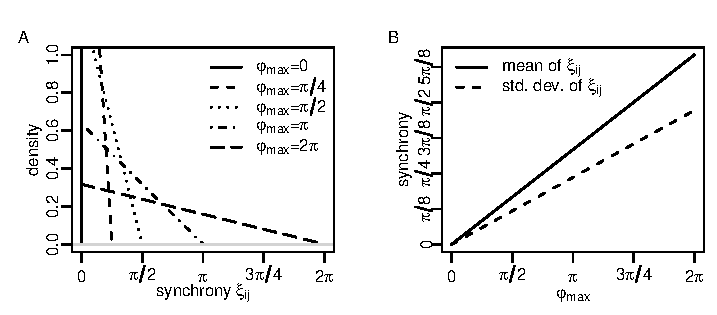
\includegraphics{figure1.pdf}
  \caption{\label{fig:synchrony}Synchrony in the case of model 0. (A) distribution of synchrony $\xi_{ij}$ for various values of $\varphi_{\mbox{\tiny max}}$. (B) mean and standard deviation of the distribution of $\xi_{ij}$ as functions of $\varphi_{\mbox{\tiny max}}$.}
\end{figure}

\bibliographystyle{plain}
\bibliography{/home/choisy/Travail/Bibliographie/Bibliographie}

\newpage
\section*{Annexe : dérivation de l'équation \ref{eq:force}}
Nous faisons l'hypothèse que le processus d'infection est fréquence-dépendent, c'est-à-dire que la force d'infection $\lambda$ est proportionnelle à une proportion d'infectés $I/N$. L'infection des susceptibles d'une population $i$ peut être due à des contacts avec des infectieux de cette même population $i$ ou à des contacts avec des infectieux d'une autre population $j$. Dans le premier cas la force d'infection s'écrit simplement
\begin{equation}
  \lambda_{i,w} = \beta_i \frac{I_i}{N_i}
\end{equation}
où $\beta$ est le taux de contat infectieux dans la population $i$. Dans le deuxième cas, un individu susceptible de la population $i$ peut s'infecter au contact d'un individu infectieux de la population $j$ de deux façons différentes : soit c'est l'individu susceptibles de la population $i$ qui va se faire infecter dans la population $j$ et reviennent dans sa population d'origine $i$, soit c'est l'individu infectieux de la population $j$ qui va infecter un individu susceptible de la population $i$ et revient dans sa population d'origine $j$. Dans la première option la force d'infection s'écrit
\begin{equation} \label{eq:bs}
  \lambda_{i,b_s} = \beta_j \frac{I_j}{N_j}
\end{equation}
et dans la deuxième option elle s'écrit
\begin{equation} \label{eq:bi}
  \lambda_{i,b_i} = \beta_i \frac{I_j}{N_i}
\end{equation}
Notez bien ici que nous nous interessons dans cette étude à la dynamique spatiale uniquement de la maladie et non pas des hôtes. Les mouvements d'individus ne sont dons pas modélisés explicitement, seule la dynamique spatiale du processus d'infection est modélisée. En combinant les équations \ref{eq:bs} et \ref{eq:bi}, la force d'infection due à des contacts avec des individus infectieux de la population voisine $j$ s'écrit
\begin{eqnarray}
  \lambda_{i,b} & = & \varepsilon \lambda_{i,b_i} + (1 - \varepsilon) \lambda_{i,b_i} \\
                & = & \varepsilon \beta_i \frac{I_j}{N_i} + (1 - \varepsilon) \beta_j \frac{I_j}{N_j} \\
                & = & \frac{\varepsilon \beta_iN_j+(1-\varepsilon)\beta_jN_i}{N_i N_j}I_j
\end{eqnarray}
où $\varepsilon$ ($0 \leqslant \varepsilon \leqslant 1$) est la proportion des infections de l'extérieur dues à des migrations d'infectés de l'extérieur, par opposition à des migrations de susceptibles de la population focale vers l'extérieur. On peut généraliser l'équation précédente au cas où l'on a $n$ populations:
\begin{equation}
  \lambda_{i,b} = \frac{1}{n-1}\sum_{\substack{
   k=1 \\
   k\neq i
  }}^{n-1}\rho_{ik}\frac{\varepsilon \beta_iN_k+(1-\varepsilon)\beta_kN_i}{N_i N_k}I_k
\end{equation}
où $\rho_{ij}=\rho_{ji}$ ($0\leqslant\rho_{ij}\leqslant1$) est la force de couplage entre les populations $i$ et $j$ : $i$ et $j$ sont totalement indépendantes si $\rho_{ij}=0$ et constituent une seule et même population homogène si $\rho_{ij}=1$.

En rajoutant à cette force d'infection la force d'infection due à des contacts avec des individus infectieux de la même population $i$ nous obtenons
\begin{eqnarray}
  \lambda_i & = & \frac{1}{2} [\lambda_{i,w} + \rho_{ij}\lambda_{i,b}] \\
            & = & \frac{1}{2} \left[\lambda_{i,w} + \rho_{ij}\frac{\varepsilon \beta_iN_j+(1-\varepsilon)\beta_jN_i}{N_i N_j}I_j\right] \label{eq:lambda_i1}
\end{eqnarray}
où $\rho_{ij}=\rho_{ji}$ ($0\leqslant\rho_{ij}\leqslant1$) est la force de couplage entre les populations $i$ et $j$ : $i$ et $j$ sont totalement indépendantes si $\rho_{ij}=0$ et constituent une seule et même population homogène si $\rho_{ij}=1$. Le facteur correctif $1/2$ rend compte du fait qu'un individu susceptible ne peut s'infecter qu'une et une seule fois. Les forces d'infections ne s'additonnent donc pas mais se moyennent. L'équation \ref{eq:lambda_i1} peut être re-écrite de la façon suivante
\begin{equation}
  \lambda_i = \frac{1}{2}\sum_{k\in\{i,j\}}\rho_{ik}\frac{\varepsilon \beta_iN_k+(1-\varepsilon)\beta_kN_i}{N_i N_k}I_k
\end{equation}
en posant $\rho_{ii}=1$. Cette dernière formulation permet de généraliser au cas où l'on a plus de deux sous-populations, ce qui donne l'équation \ref{eq:force}:
$$
  \lambda_i = \frac{1}{n}\sum_{j=1}^n\rho_{ij}\frac{\varepsilon \beta_iN_j+(1-\varepsilon)\beta_jN_i}{N_i N_j}I_j
$$
où $n$ est le nombre de sous-populations.

\hfill$\square$

\end{document}
